\chapter{Methodology}\label{ch:Methodology}

\subsection{Original Neural Radiance Fields (NeRF)}
Neural Radiance Fields (NeRF) \cite{Mildenhall2020} as a foundational notion established a new paradigm for scene representation. The main concept is to describe a scene as a continuous, high-dimensional radiance field, $F_\Theta$, where $\Theta$ represents the multilayer perceptron's (MLP) parameters. NeRF is based on computer graphics theory and uses deep learning methods to produce synthesized views with previously unheard-of levels of photorealism. In Figure \ref{fig:Original NERF Overview}, an overview of NeRF is presented. On the left side of the image, the black dots indicate areas where the network has not yet learned any color information. In contrast, the second image demonstrates the colored output corresponding to a single pixel.

\begin{figure}[thbp]
    \centering
    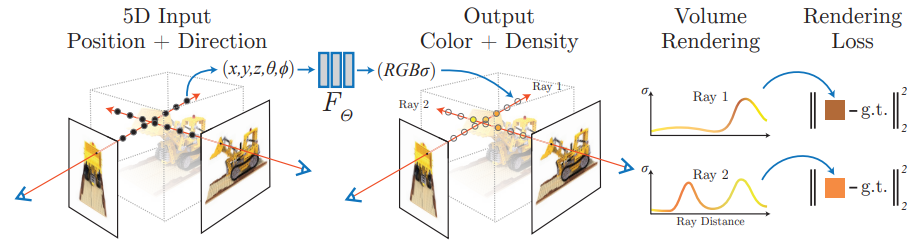
\includegraphics[width=.9\textwidth]{img/Original Nerf.png}
    \caption{NeRF Overview: Image creation involves sampling 5D coordinates along camera rays, using a multilayer perceptron for color and density, and employing volume rendering for image compilation \cite{Mildenhall2020}.
}\label{fig:Original NERF Overview}
\end{figure}

Given any 3D location in space $\mathbf{x} = (x, y, z)$ and a specific 2D viewing direction $\mathbf{d} = (\theta, \phi)$, the MLP is designed to output both an RGB color vector $\mathbf{c} = (r, g, b)$ and a scalar volume density $\sigma$ \cite{Mildenhall2020}. This relationship is mathematically expressed as:

$$F_\Theta: (\mathbf{x}, \mathbf{d}) \rightarrow (\mathbf{c}, \sigma)$$

Where:
\begin{itemize}
    \item $F_{\theta}$ is the neural radiance field parameterized by network parameters $\theta$.
    \item $\mathbf{x} = (x, y, z)$ represents the 3D coordinates.
    \item $\mathbf{d} = (\theta, \phi)$ denotes the 2D viewing direction.
    \item $\mathbf{c} = (r, g, b)$ is the emitted color.
    \item $\sigma$ is the volume density.
\end{itemize}


Volumetric ray marching is used in NeRF\cite{Mildenhall2020} to accomplish the rendering process. Using this method, rays are traced into the scene from the camera origin, and sampling points are taken along each ray. The MLP is contacted at each of these sample places in order to get density and color values. An alpha compositing technique is used to accumulate color along a ray. This can be stated as:


$$C(\mathbf{r}) = \sum_{i=1}^{N} T_i (1 - \exp(-\sigma_i \delta_i)) \mathbf{c}_i,$$

where $T_i = \exp(- \sum_{j=1}^{i-1} \sigma_j \delta_j)$ represents\cite{Mildenhall2020} the transmittance, accounting for the absorption and scattering of light as it travels through the medium. Here, $\delta_i$ denotes the distance between adjacent sampled points along the ray.

\vspace{10pt}
Reconstruction loss vs rendered loss is used to optimize the whole NeRF model by reducing the discrepancy between rendered and captured views. Through this optimization, the MLP is able to pick up on both geometric and photometric subtleties, resulting in a very accurate and detailed representation of the scene.


\subsection{Extending NeRF to Handle Transmission Electron Microscopy (TEM) Data}
The standard NeRF pipeline relies on accurate camera pose estimation, typically obtained through structure-from-motion methods like COLMAP. However, TEM images pose challenges due to their noise levels and unique characteristics, making traditional pose estimation techniques like COLMAP ineffective.

\vspace{10pt}
\begin{figure}[thbp]
    \centering
    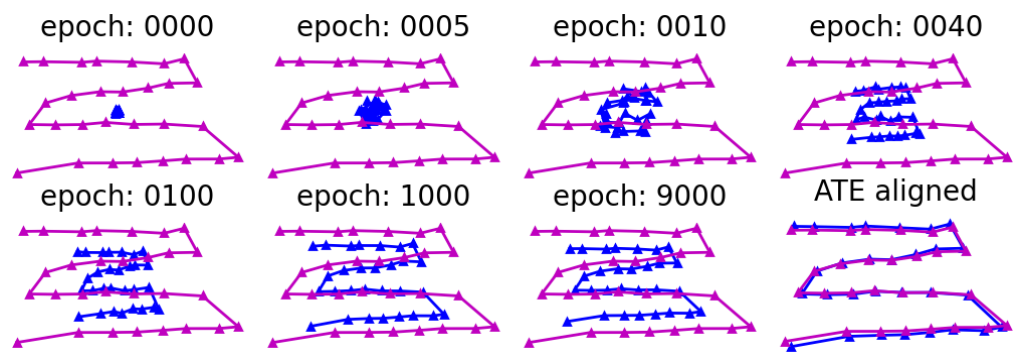
\includegraphics[width=.9\textwidth]{img/Colmap_nerfMM.png}
    \caption{Optimization of Camera Pose in NeRF-MM. The purple path represents the camera trajectory derived from COLMAP, while the blue path illustrates the camera trajectory as determined by NeRF-MM. \cite{Wang2021}
}\label{fig: Camera pose comparison NerfMM}
\end{figure}

\label{fig:Dataset_3_with_Tanh_10000_epochs.jpg}
Introduced by Wang et al. in 2021 \cite{Wang2021}, NeRF-MM (Neural Radiance Fields Without Known Camera Parameters) represents a substantial advancement of the original NeRF model. This enhanced version is tailored to address the intricacies involved in generating camera poses during training, as depicted in \ref{fig: Camera pose comparison NerfMM}. Such a feature is especially relevant in the realm of TEM (Transmission Electron Microscopy) imaging, where accurately determining camera positions is crucial.

\vspace{10pt}

The primary innovation in NeRF-MM is its capability to process and interpret multimodal data. This is achieved by incorporating additional scene descriptors or feature vectors for each 3D point in the space. This approach is crucial in TEM imaging, where different materials can exhibit varied electron interactions, significantly impacting the final image quality.

\vspace{10pt}
NeRF-MM introduces a conditioning model, \( C_\Phi \), which is central to its ability to handle multimodal data. The conditioning model is defined as:

\begin{equation}
C_\Phi: \mathbf{x} \rightarrow \mathbf{f}
\end{equation}

Where \( \mathbf{x} \) is the 3D coordinate in the scene, and \( \mathbf{f} \) represents the generated feature vector. This vector encodes additional information about the scene, such as material properties or lighting conditions, which are not captured by the spatial coordinates alone.

\vspace{20pt}

The radiance field function in NeRF-MM is modified to incorporate these feature vectors:

\begin{equation}
F_\Theta: (\mathbf{x}, \mathbf{d}, \mathbf{f}) \rightarrow (\mathbf{c}, \sigma)
\end{equation}

Here, \( \mathbf{d} \) represents the viewing direction. The function outputs the color \( \mathbf{c} \) and density \( \sigma \) at the point \( \mathbf{x} \), considering the feature vector \( \mathbf{f} \) and viewing direction \( \mathbf{d} \).

\vspace{10pt}
A critical aspect of NeRF-MM is its advanced approach to volumetric integration. The model employs a sophisticated sampling strategy along the rays passing through the scene. This is mathematically represented as:

\begin{equation}
\text{Color}(\mathbf{r}) = \int_{t_n}^{t_f} T(t) \sigma(\mathbf{r}(t)) \mathbf{c}(\mathbf{r}(t), \mathbf{d}) dt
\end{equation}

In this equation, \( T(t) \) denotes the accumulated transmittance along a ray \( \mathbf{r} \) from the near boundary \( t_n \) to the far boundary \( t_f \) \cite{Wang2021}. This intricate sampling method ensures a detailed and accurate reconstruction of the scene, which is especially beneficial in TEM imaging where the subjects often exhibit complex geometries and material properties.

\vspace{10pt}

To optimize NeRF-MM for the specific challenges of TEM imaging, such as high noise levels and fine-scale detail capture, we have introduced targeted modifications to the model. These include:

\begin{itemize}
  \item Changing the MLP's width and depth will improve the model's ability to handle complicated structures that are common in TEM data.
  \item Fine-tuning the conditioning model \( C_\Phi \) to better represent the unique material properties encountered in TEM imaging.
  \item Implementing a noise-aware training strategy to improve the model's robustness to the high noise levels commonly found in TEM datasets.
\end{itemize}


A notable feature of NeRF-MM is its independence from external camera parameter estimation tools, such as COLMAP. This is particularly advantageous in TEM imaging, where precise camera positioning and calibration can be challenging. NeRF-MM's advanced feature vector representation and sampling methods allow it to inherently adapt to scenes with minimal or no camera parameter information, facilitating its application in TEM imaging.


\vspace{10pt}

NeRF-MM, with its advanced architecture and multimodal data handling capabilities, represents a significant evolution in the field of 3D reconstruction, particularly for TEM imaging. Its unique approach to incorporating additional scene descriptors, sophisticated volumetric integration, and optimizations tailored for TEM data, make it an ideal choice for addressing the challenges inherent in TEM imaging scenarios. By effectively capturing and processing the complex interplay of material properties and electron beam interactions, NeRF-MM enables the creation of highly detailed and accurate 3D models from TEM datasets.


\vspace{20pt}
\textbf{Adopting NeRF-Dark Techniques:} NeRF-Dark, as proposed by Mildenhall et al. in 2021 \cite{Mildenhall2021}, marked a significant advancement in handling low-light conditions, a feature beneficial for TEM imaging where illumination is often limited. Building on this, RawNeRF, a variation trained on linear raw images, demonstrates remarkable capabilities in reconstructing scenes from extremely noisy images captured in near-dark conditions. This makes it particularly suitable for the challenges faced in TEM imaging.

\vspace{10pt}
NeRF in the Dark referred as RawNeRF outperforms conventional single and multi-image deep raw denoisers by effectively combining information from all input images for reconstruction \cite{Mildenhall2021}, even in the absence of explicitly learned image priors or clean training data. This approach allows RawNeRF to serve as a powerful multi-image denoiser for wide-baseline static scenes, efficiently aggregating observations from widely spaced input images. Moreover, the linear High Dynamic Range (HDR) scene representation of RawNeRF supports novel view synthesis tasks, including adjustments in focus, exposure, and tonemapping post-rendering. This flexibility is a significant leap forward in scene reconstruction and view synthesis \cite{Mildenhall2021}.

\vspace{10pt}

RawNeRF demonstrates exceptional noise robustness, handling high levels of image noise and surpassing traditional NeRF and other denoising methods in producing accurate scene representations. This capability makes it particularly effective for TEM imaging, which often contends with significant noise challenges. Merging principles from NeRF, low-level image processing, and HDR imaging, RawNeRF contributes substantially to advancements in scene reconstruction and view synthesis. Utilizing this interdisciplinary approach, we have integrated RawNeRF's denoising methodology into our updated NerfMM variant. This integration not only enables the 3D reconstruction of TEM images but also enhances denoising capabilities, surpassing the performance of NerfMM alone. This synergy ensures high-quality image reconstruction from TEM data, typically challenged by darkness and noise.

\vspace{10pt}

\textbf{Utilizing NAN-NeRF Innovations:} 
NAN-NeRF, a breakthrough by Pearl et al. in 2022 \cite{Pearl2022}, marks a significant advancement in NeRF's application to nanoscale imaging, a domain closely aligned with TEM that often grapples with capturing fine details at a small scale. This innovation is particularly relevant for our methodology, addressing TEM's challenges in resolving intricate details at the nanoscale. NAN-NeRF excels in reconstructing accurate 3D models from highly limited and noisy data, a capability crucial for TEM, where data quality and quantity are often limited due to sample sensitivity and electron dose constraints.

\vspace{10pt}
In our approach, we've adopted key techniques from NAN-NeRF, such as replacing NerfMM's ReLU function with NAN-NeRF's Leaky ReLU and Sigmoid functions. Additionally, we've implemented separate Adam optimizers for NerfMM and other parameters from NAN-NeRF. These modifications are tailored to enhance our methodology, aiming to achieve more precise 3D reconstructions and better handle the intricate challenges posed by TEM imaging at the nanoscale. This integration of NAN-NeRF techniques into our framework not only improves the denoising capabilities but also ensures a more nuanced and detailed approach to reconstructing high-quality images from TEM data.

\vspace{10pt}

\textbf{Hyperparameter Adjustments for TEM Data:} 
In response to the lower signal-to-noise ratio typical of TEM images, our methodology incorporates essential hyperparameter adjustments in the NeRF model to enhance sensitivity to subtle data variations, crucial for distinguishing actual features from noise. Key modifications include a refined learning rate for more precise model updates, and adjustments to the depth and width of the NeRF model's MLP to balance modeling complex TEM structures and avoiding noise overfitting. Advanced denoising techniques and exposure correction algorithms are also employed to improve feature visibility in low-light TEM images.

\vspace{10pt}
Our experimentation extended to a comprehensive tuning of all possible hyperparameters to optimize the model for TEM imaging. We incorporated activation functions from NAN-NeRF and fine-tuned network layers to achieve the best results. To validate the model's accuracy, we reserved one sample image with a known camera position, separate from the training set. We also adopted different optimization algorithms from NAN-NeRF. While the best results were obtained at 10,000 epochs, this was time-intensive, taking approximately 10 to 14 hours. Therefore, for baseline experiments, we opted for 200 to 1000 epochs, which significantly reduced processing time to a few minutes to an hour. After establishing successful baseline results, we conducted all experiments at 10,000 epochs to maximize accuracy and detail in the reconstructed images.


\vspace{10pt}

In summary, by integrating these advanced NeRF variations and meticulously adjusting hyperparameters, our methodology establishes a robust framework for handling the noise and imaging challenges characteristic of TEM data. This approach not only enhances the fidelity and quality of TEM imaging but also broadens the scope of its applications in material science and nanotechnology research.

\subsection{Post-Reconstruction Processing with ESRGAN}
In the post-reconstruction phase of our TEM imaging analysis, the 3D model's frames undergo further processing for denoising. Among various methods explored, Enhanced Super-Resolution Generative Adversarial Networks (ESRGAN)\cite{Xintao2018} proved to be exceptionally effective. The ESRGAN model operates by transforming a low-resolution, noisy input image into a high-resolution, denoised output. 
\vspace{10pt}

The ESRGAN model utilizes a generative adversarial network (GAN) framework comprising a generator and a discriminator, trained simultaneously. The generator aims to produce images that closely resemble real, high-resolution images, while the discriminator evaluates their authenticity. Through this adversarial training, ESRGAN learns to enhance details and reduce noise effectively. It incorporates advanced loss functions, including perceptual and adversarial loss, to improve image quality and detail fidelity. This capability makes ESRGAN particularly adept at handling the complex textures and subtle details characteristic of TEM imagery, thereby significantly enhancing the quality and utility of the reconstructed models.


\vspace{10pt}
\textbf{Implementation of ESRGAN in Our Workflow:} In our methodology, the application of ESRGAN is a principal post-processing step after extracting frames from the 3D model. However, we designed this step to be flexible, allowing for the possibility of incorporating other advanced methods in the future. Our decision to use ESRGAN was based on comprehensive trials involving various GANs and denoising techniques. Among these, ESRGAN stood out for its exceptional performance in enhancing a specific dataset we evaluated. Its proficiency in preserving and recovering intricate details, coupled with its effective noise reduction, was instrumental in our choice to integrate it into our workflow.

\vspace{10pt}
\textbf{Performance Metrics and Results:} The proficiency of ESRGAN is quantifiably demonstrated through its remarkable performance in peak signal-to-noise ratio (PSNR) and Structural Similarity Index Measure (SSIM) metrics. In our evaluations, ESRGAN achieved a PSNR of 38.70, outperforming other methods, and recorded an SSIM value of 0.95. These metrics are especially significant in TEM imaging, as they are directly indicative of the clarity and accuracy of the reconstructed images.



\vspace{10pt}
\subsection{Integrating Traditional Denoising Techniques}
In addition to advanced techniques like ESRGAN, traditional denoising methods also play a significant role in post-processing the frames of the 3D model. These methods are essential for handling various types of noise and artifacts present in the images.
\vspace{10pt}

Traditional denoising techniques employed include wavelet denoising, Gaussian blur, median filtering, bilateral filtering, and non-local means denoising. Each method offers unique advantages in reducing noise while preserving the essential features of the image.

\begin{itemize}
    \item \textbf{Wavelet Denoising}: This method employs wavelet transforms to decompose an image into various frequency components. By selectively thresholding these components, it effectively separates noise from significant image features. Wavelet denoising is particularly effective for TEM images with non-uniform noise distribution or images where noise characteristics vary across different regions.
    
    \item \textbf{Gaussian Blur:} Gaussian blur involves convolving the image with a Gaussian kernel. This process smooths the overall image, reducing high-frequency noise elements like grainy textures. It's especially useful in TEM images where the primary concern is overall image graininess rather than preserving high-frequency details.

    \item \textbf{Median Filtering:} In median filtering, each pixel is replaced with the median value of its surrounding pixels. This technique is particularly effective in removing 'salt-and-pepper' noise, common in digital image sensors and often encountered in TEM imaging.
    
    \item \textbf{Bilateral Filtering:} Bilateral filtering is a more sophisticated approach that combines smoothing with edge preservation. By considering both spatial and intensity differences, it smooths the image while maintaining edge details, making it suitable for TEM images where edge preservation is crucial.
    
    \item \textbf{Non-Local Means Denoising:} This technique works by averaging similar patches across the image, thus preserving textures and details. It's particularly effective in TEM imaging for maintaining structural integrity in the presence of noise, as it does not rely on local neighborhood intensity values alone.
    
\end{itemize}

These methods were systematically applied to the frames extracted from the 3D model. The process involved reading each frame, applying the denoising techniques, and saving the enhanced images into respective subfolders for each method. This method made sure that the best denoising technique could be chosen according to the unique properties of the noise in every frame.



\subsection{Adapted Framework for TEM Data Analysis}

In summary, the methodology presented in this chapter represents a pioneering convergence of advanced computational techniques and traditional image processing methods, specifically tailored for the unique challenges of Transmission Electron Microscopy (TEM) data analysis. By integrating state-of-the-art Neural Radiance Fields (NeRF) models with a combination of modern and traditional denoising strategies, we have established a comprehensive framework that significantly enhances the quality and usability of TEM data.

\begin{figure}[thbp]
    \centering
    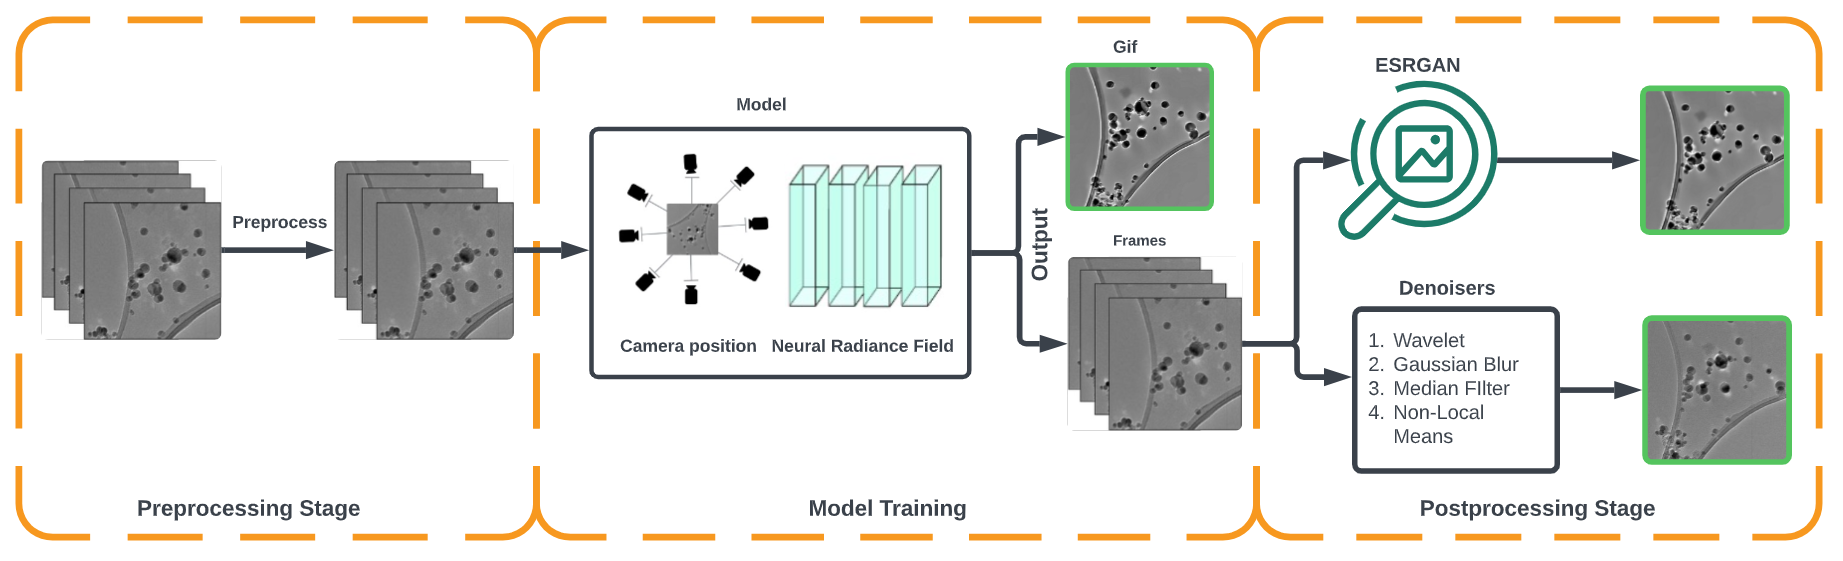
\includegraphics[width=\textwidth]{img/Thesis Architecture Image.png}
    \caption{Comprehensive overview of our framework: Integrating NeRF and advanced Denoising Techniques, ESRGAN for Enhanced TEM Image Analysis}
    \label{fig:ThesisArchitecture}
\end{figure}

As depicted in Figure \ref{fig:ThesisArchitecture}, our framework illustrates the power of integrating diverse computational methodologies into a cohesive process. The \textbf{green} borders in the architecture diagram highlight three key outcomes:

\begin{enumerate}
    \item \textbf{3D Reconstruction from 2D Input Images:} The first green-bordered image represents the transformation of traditional 2D TEM data into comprehensive 3D models using NeRF, providing deeper insights into material structures.
    \item \textbf{Output from ESRGAN:} The second green-bordered image showcases the enhanced output from the application of ESRGAN, focusing on resolution enhancement and noise reduction in TEM images.
    \item \textbf{Optimal PSNR from Traditional Denoising Algorithms:} The final green-bordered image represents the best result achieved using traditional denoising algorithms, emphasizing the importance of these techniques in preserving image fidelity.
\end{enumerate}


